\documentclass[11pt, oneside]{article}	% use "amsart" instead of "article" for AMSLaTeX format
\usepackage{geometry}	
%\usepackage[utf8]{inputenc}
\usepackage{hyperref}

% See geometry.pdf to learn the layout options. There are lots.

\geometry{a4paper}								% ... or letterpaper or a5paper or ... 
%\usepackage{relsize}
\usepackage{amsmath}
%\geometry{landscape}							% Activate for rotated page geometry
%\usepackage[parfill]{parskip}				% Activate to begin paragraphs with an empty line rather than an indent
\usepackage{graphicx}							% Use pdf, png, jpg, or eps§ with pdflatex; use eps in DVI mode
%\usepackage[dvipdfmx]{graphicx} 
\usepackage{bmpsize} 

%\usepackage{luamplib}

% TeX will automatically convert eps --> pdf in pdflatex		
\usepackage{amssymb}
%SetFonts

\usepackage{float}

\title{WEIBULL: $W_{pdf}$ maximum likelihood estimation, analysis}
\author{D Palahnuk}
%\date{}										% Activate to display a given date or no date
\usepackage{comment}


\begin{document}
	\maketitle
	
	%\section{}
	%\subsection{}




	
\textbf{For Weibull - We apply the MLE calculation:} \\


We start by assuming Weibull pdf that is ``Independent Identically Distributed'' which is usually designated as i.i.d. (or perhaps Markov depending on how you define or scope the analysis): 

$$
X = \left\{x_{1}, \ldots, x_{n}\right\}, \quad W{_{pdf}}(k, \lambda)
$$






$$
f(x ; \lambda, k)= \begin{cases}\frac{k}{\lambda}\left(\frac{x}{\lambda}\right)^{k-1} e^{-(x / \lambda)^{k}}, & x \geq 0 \\ 0, & x<0\end{cases}
$$




$$
L\left(\Theta \mid X \right)= L\left(x_{1}, \cdots x_{n} ; \gamma, \theta\right)=\prod_{i=1}^{n}(\gamma / \theta) x_{i}^{\gamma-1} \exp \left(-x_{i}^{\gamma} / \theta\right)
$$

Consider the maximum of $\log \left(L\left(\Theta \mid X \right)\right)$:\\

$$
\frac{\partial (\log L\left(\Theta \mid X \right))}{\partial \gamma}=0 
\quad and \quad
\frac{\partial (\log L\left(\Theta \mid X \right))}{\partial \theta}=0 
\quad and \quad 
$$\\

Solving the first order differentials:\\

$$
\frac{\partial \ln L}{\partial \gamma}=\frac{n}{\gamma}+\sum_{1}^{n} \ln x_{i}-\frac{1}{\theta} \sum_{1}^{n} x_{i}^{\gamma} \ln x_{i}=0
$$

$$
\frac{\partial \ln L}{\partial \theta}=-\frac{n}{\theta}+\frac{1}{\theta^{2}} \sum_{1}^{n} x_{i}^{\gamma} \quad=0
$$

On eliminating $\theta$ between these two equations and simplifying, we have
$$
\left[\frac{\sum_{1}^{n} x_{i}^{\gamma} \ln x_{i}}{\sum_{1}^{n} x_{i}^{\gamma}}-\frac{1}{\gamma}\right]=\frac{1}{n} \sum_{1}^{n} \ln x_{i},
$$


\noindent
We have to now solve the MLE for the best estimate of $\hat{\gamma}$. There is no analytic closed solution here for $\hat{\gamma}$, unfortunately. However, this can be solved by iteration, or trial and error. Once two values $\gamma_{1}$ and $\gamma_{2}$ have been found in an interval such that $\gamma_{1}<\gamma<\gamma_{2}$, end with a linear interpolation for $\hat{\gamma}$.\\




With $\hat{\gamma}$ thus determined, $\theta$ is estimated as

$$
\hat{\theta}=\sum_{1}^{n} x_{i}^{\hat{\gamma}} / n
$$
\noindent
INterestingly enough - this simply looks like the average of the $x_{i}$ at some power $\hat{\gamma}$.





\newpage
*Discussion*\\ 

This data is what I like to refere to a ceiling (or floor) data - in other words the data ranges to 100 (or 0) percent. In this example it is a cell culture viability distribution. Therefore, it won't be normally distributed. This type of distribution is often seen in the Biotech area - where we have a top 100 percent value as a ceiling.\\

We have a few choices: Transform it, do it non-parametrically, or use a suitable pdf. In this case the Weibull pdf is used since the shape is reasonable. Here we set the LSL (spec limit) to 80 percent. And it shows a calculated Ppk of 3.9 ... showing the spec limit may be able to be raised based on the process ANOVA for the viability for the expample vial thaw.\\ 

VIAL THAW Viability Distribution ANOVA: For the purposes of a NON-Normal distibution in Cpk type capability analysis. This follows from applying a Weibull pdf approach and is supported by MLE theory (roughly) derived above. 

\begin{figure}[H]
\centering
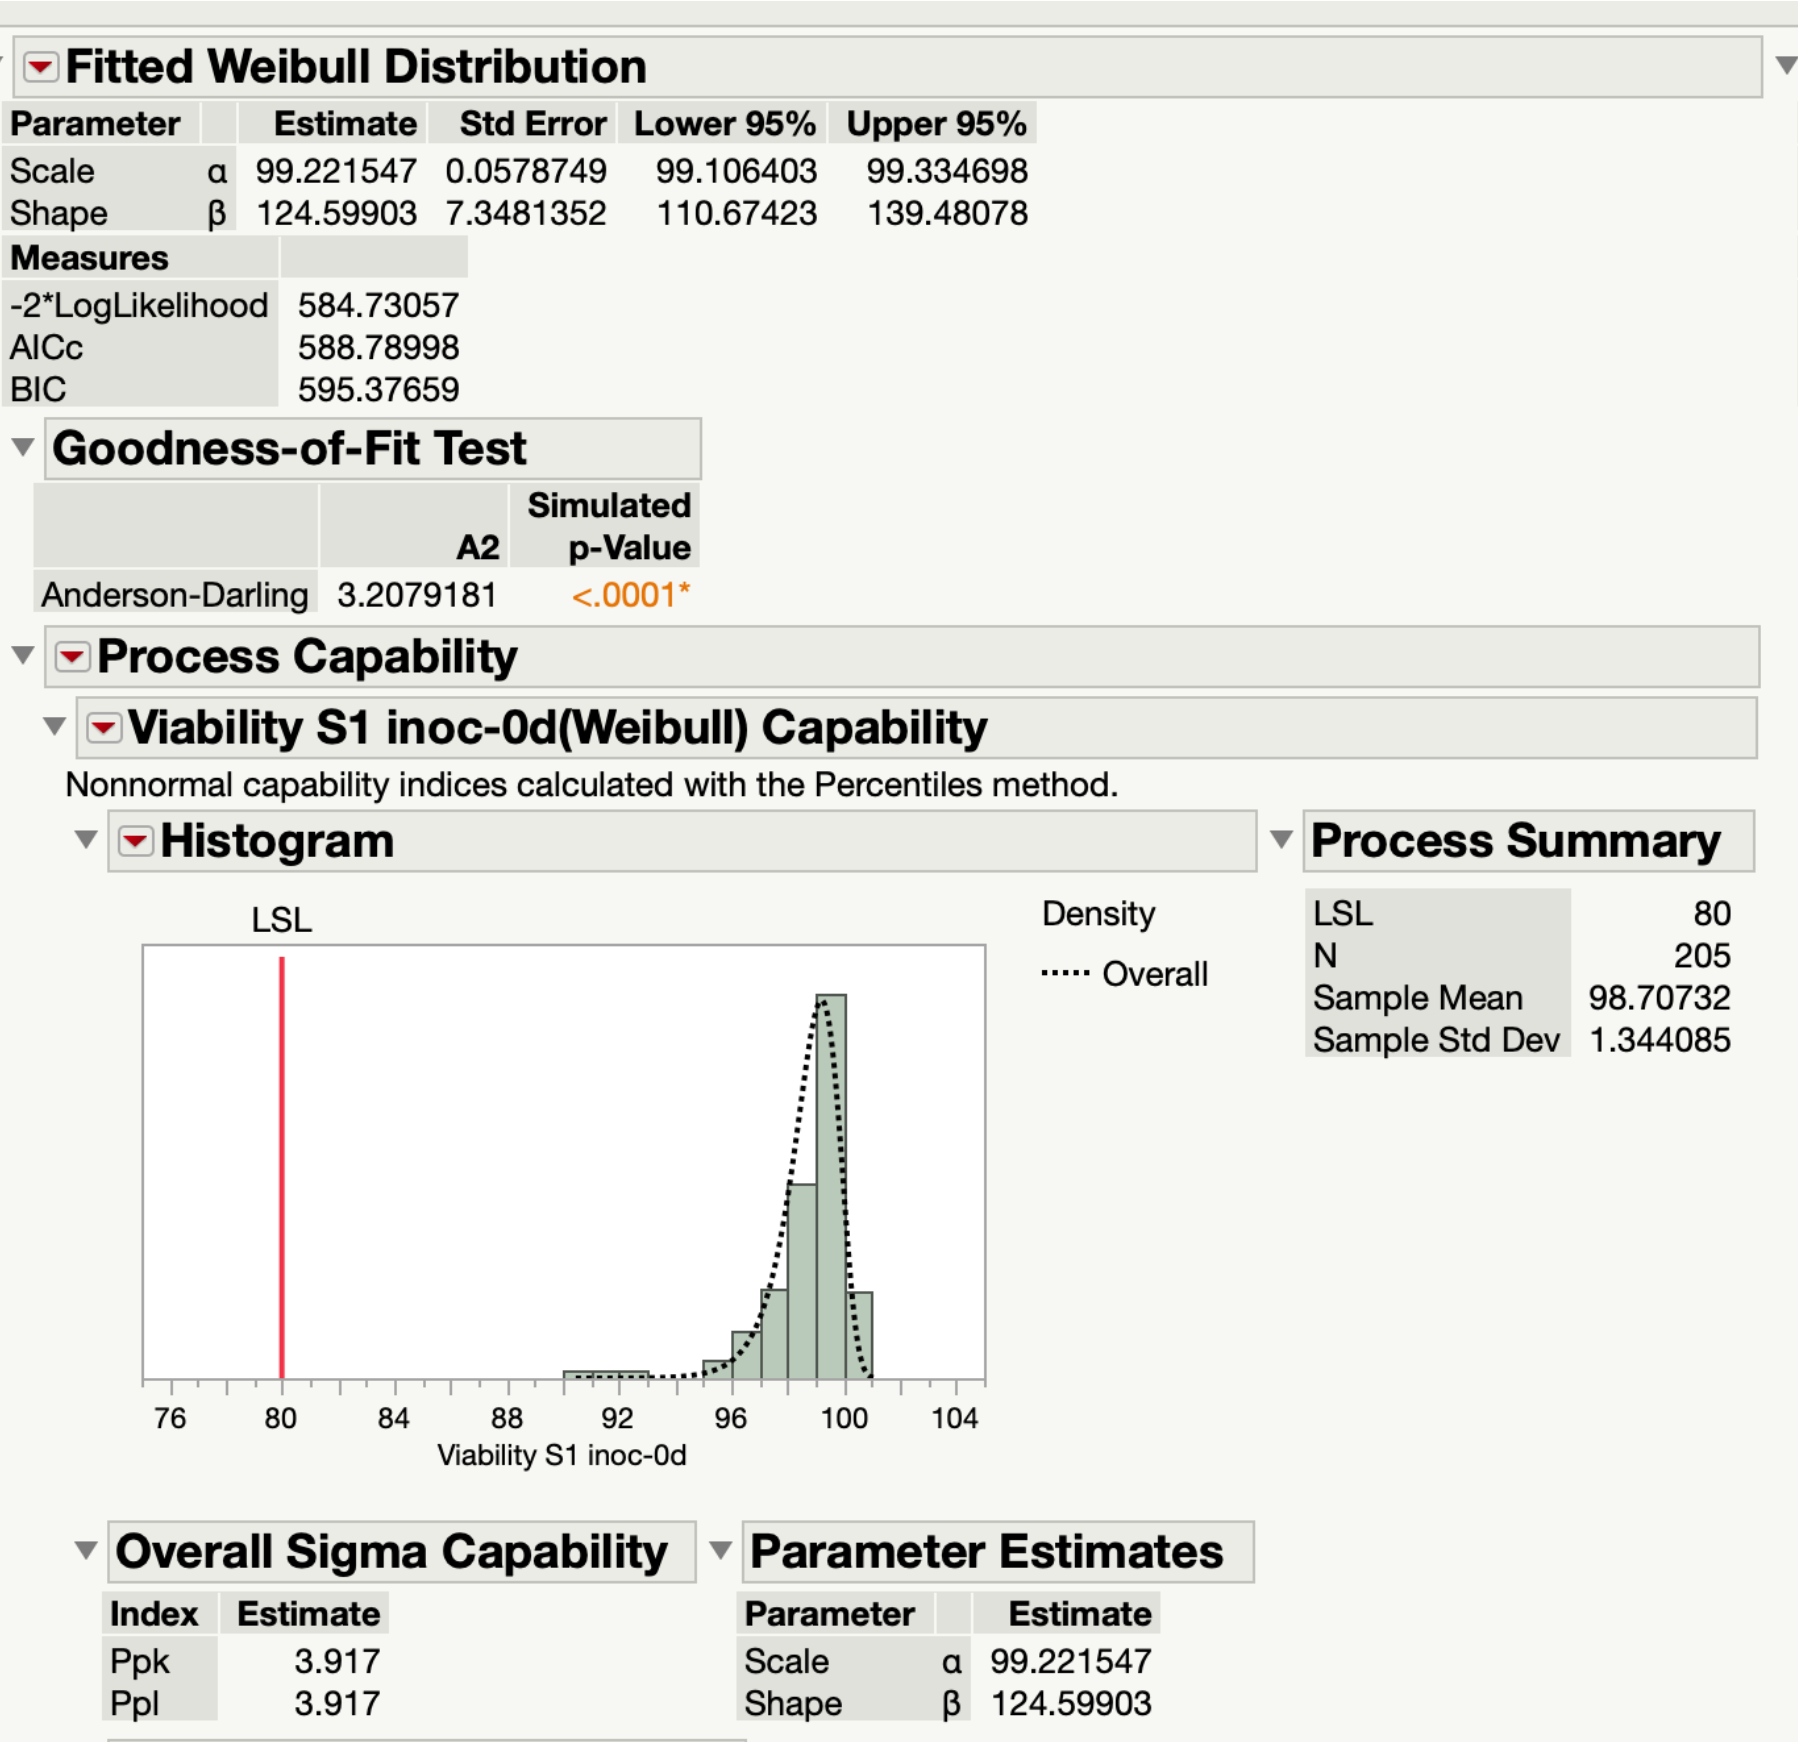
\includegraphics[scale=0.35]{Anova Weibull JS1 seed Example.png}
\end{figure}



\begin{comment}

Recall we can expand the product by  using use some simple ``nifty'' identities for the log function and sum of exponents: 
$$
\begin{aligned}
\log(a \times b) &= \log(a) + \log(b)\\
\prod_{i=1}^{n} p^{x_{i}}&=p^{\sum x_{i}} \\
\log \left(p^{a}\right)&=a \log (p) \\
\log \left(p^{a+b}\right)&=a \log (p)+b \log (p) \\
\log \left(\prod_{i=1}^{n} p^{x_{i}}\right)&=\sum_{i=1}^{n} x_{i} \log (p)\\ 
\log (e) &= 1
\end{aligned}
$$
Taking the log of the likelihood function (for ease of $1^{st}$ order derivative minimization):

$$
\log ( \prod_{i=1}^{n} f_{X}(x ; \mu, \sigma))
$$

$$
=\log \left(\frac{1}{\sqrt{2 \pi \sigma^{2}}} e^{-\left(x_{1}-\mu\right)^{2} / 2 \sigma^{2}} \times \ldots \times \frac{1}{\sqrt{2 \pi \sigma^{2}}} e^{-\left(x_{n}-\mu\right)^{2} / 2 \sigma^{2}}\right)
$$

$$
=\log \left(\frac{1}{\sqrt{2 \pi \sigma^{2}}} e^{-\left(x_{1}-\mu\right)^{2} / 2 \sigma^{2}}\right)+\ldots+\log \left(\frac{1}{\sqrt{2 \pi \sigma^{2}}} e^{-\left(x_{n}-\mu\right)^{2} / 2 \sigma^{2}}\right)
$$\\
Now note specifically for $x_{1}$: 
$$
\log \left(\frac{1}{\sqrt{2 \pi \sigma^{2}}} \times e^{-\left(x_{1}-\mu\right)^{2} / 2 \sigma^{2}}\right)
$$

$$=\overbrace{\log \left(\frac{1}{\sqrt{2 \pi \sigma^{2}}}\right)+ \log \left(e^{-\left(x_{1}-\mu\right)^{2} / 2 \sigma^{2}}\right)}^{\log(a \times b) = \log(a) + \log(b}
$$

$$=\log \left[\left(2 \pi \sigma^{2}\right)^{-1 / 2}\right] - \overbrace{ \frac{\left(x_{1}-\mu\right)^{2}}{2 \sigma^{2}} \log (e)}^{\log \left(p^{a}\right) =a \log (p)}
$$

$$
 = -\frac{1}{2} \log \left(2 \pi \sigma^{2}\right) -\frac{\left(x_{1}-\mu\right)^{2}}{2 \sigma^{2}} = -\frac{1}{2} \log (2 \pi)-\frac{1}{2} \log \left(\sigma^{2}\right)-\frac{\left(x_{1}-\mu\right)^{2}}{2 \sigma^{2}}
$$ 
$$
= -\frac{1}{2} \log (2 \pi)-\log (\sigma)-\frac{\left(x_{1}-\mu\right)^{2}}{2 \sigma^{2}}
$$\\

Which gives us a easier to handle MLE objective function for differentiation: 

By summing over all n samples for $x_{i}$: 

$$
\log \left[L\left(\mu, \sigma \mid x_{1}, \ldots, x_{n}\right)\right]
$$


$$
\begin{gathered}
=-\frac{1}{2} \log (2 \pi)-\log (\sigma)-\frac{\left(x_{1}-\mu\right)^{2}}{2 \sigma^{2}}
-\ldots-\frac{1}{2} \log (2 \pi)-\log (\sigma)-\frac{\left(x_{n}-\mu\right)^{2}}{2 \sigma^{2}}
\end{gathered}
$$

$$
=-\frac{n}{2} \log (2 \pi)-n \log (\sigma)-\frac{\left(x_{1}-\mu\right)^{2}}{2 \sigma^{2}}-\ldots-\frac{\left(x_{n}-\mu\right)^{2}}{2 \sigma^{2}}
$$\\


Both the mean and the variance are UNKNOWN - and we want to estimate them on the basis of these observations ! We want to determine the proper  $\mu$, and $ v$ based on the data. Who wadda thunk ... LOL \\

Note that the term $x$ is a `vector'\\ 

$
\text {We seek to minimize this expression: } $
$$
-\frac{n}{2} \log (2 \pi)- n \log \sigma -\sum_{i=1}^{n} \frac{\left(x_{i}-\mu\right)^{2}}{2 \sigma^{2}}
$$\\


$
\text {We minimize w.r.t. } \mu \text {, }
$
to obtain the estimate of the mean:

$$
\frac{\partial}{\partial \mu} \log \left[L\left(\mu, \sigma \mid x_{1}, \ldots, x_{n}\right)\right] = 0
$$


$$
\frac{\partial \left( \frac{n}{2} \log (2 \pi) + {n} \log \sigma+\sum_{i=1}^{n} \frac{\left(x_{i}-\mu\right)^{2}}{2 \sigma^{2}}\right)}{\partial \mu}= 0
$$
$$
=0-0+\frac{\left(x_{1}-\mu\right)}{\sigma^{2}}+\ldots+\frac{\left(x_{n}-\mu\right)}{\sigma^{2}}
$$



$$
=\frac{1}{\sigma^{2}}\left[\left(x_{1}+\ldots+x_{n}\right)-n \mu\right]=0
$$

$$
\frac{1}{\sigma^{2}} \sum_{i=1}^{n} \left(x_{i}-\mu\right)=0 ~~~~ \Rightarrow ~~~~ \sum_{i=1}^{n}  x_{i}=n \mu ~~~~ \Rightarrow ~~~~ \widehat{\mu}=\frac{x_{1}+\cdots+x_{n}}{n}
$$\\

$
\text {We minimize w.r.t. } \sigma \text {, }
$
to obtain the estimate of the variance:

$$
\frac{\partial}{\partial \sigma} \log \left[L\left(\mu, \sigma \mid x_{1}, \ldots, x_{n}\right)\right] = 0
$$


$$
\frac{\partial \left( \frac{n}{2} \log (2 \pi) + {n} \log \sigma+\sum_{i=1}^{n} \frac{\left(x_{i}-\mu\right)^{2}}{2 \sigma}\right)}{\partial \sigma}= 0
$$

$$
=0-\frac{n}{\sigma} -\sum_{i=1}^{n}\frac{\left(x_{i}-\mu\right)^{2}}{2}(-2) \sigma^{-3} = 0
$$

$$
\frac{n}{\sigma}+\sum_{i=1}^{n}\frac{\left(x_{1}-\mu\right)^{2}}{\sigma^{3}} = 0 
$$


$$
\begin{aligned}
&0=-n+\frac{1}{\sigma^{2}}\left[\left(x_{1}-\mu\right)^{2}+\ldots+\left(x_{n}-\mu\right)^{2}\right] \\
&n=\frac{1}{\sigma^{2}}\left[\left(x_{1}-\mu\right)^{2}+\ldots+\left(x_{n}-\mu\right)^{2}\right] \\
&n \sigma^{2}=\left(x_{1}-\mu\right)^{2}+\ldots+\left(x_{n}-\mu\right)^{2}
\end{aligned}
$$


$$
\sigma^{2} \cdot n -\sum_{i=1}^{n} \left(x_{i}-\mu\right)^{2}=0 ~~~ \Rightarrow ~~~ \widehat{\sigma}=\sqrt{\frac{1}{n} \sum_{i=1}^{n}\left(x_{i}-\widehat{\mu}\right)^{2}}
$$


$$
\widehat{\sigma}=\sqrt{\frac{\left(x_{1}-\mu\right)^{2}+\ldots+\left(x_{n}-\mu\right)^{2}}{n}}
$$


\newpage

Thus maximum of the MLE $L\left(\Theta \mid X \right)$, or in this case:  $\log \left(L\left(\Theta \mid X \right)\right)$, for
$$
\quad f_{X}(x ; \mu, \sigma)= \frac{1}{\sqrt{2 \pi \sigma}} \exp \left\{-\frac{\left(x-\mu\right)^{2}}{2 \sigma}\right\}
$$
 results in the estimate for the mean $\mu$ and the standard deviation $\sigma$.\\

$$
\Rightarrow ~~~~ \widehat{\mu}=\frac{x_{1}+\cdots+x_{n}}{n}
$$\\

$$
\Rightarrow ~~~~ \widehat{\sigma}=\sqrt{\frac{\left(x_{1}-\mu\right)^{2}+\ldots+\left(x_{n}-\mu\right)^{2}}{n}}
$$


\begin{figure}[H]
\centering
\includegraphics[scale=0.3]{mle result Npdf.png}
\end{figure}

\end{comment}
	
\end{document}  



















